\documentclass[18pt]{beamer}
\usepackage[utf8]{inputenc}
\usepackage{templates/mytemplate}
\usepackage{templates/beamerthemekit}
\usepackage{graphicx}
\usepackage{microtype}
\usepackage{listings}
\usepackage{color}
\usepackage{hyperref}
\usepackage{multicol}
\usepackage{siunitx}
\usepackage{physics}
\usepackage{appendixnumberbeamer}

\title{Difference in Kinematic Distributions of GCR August  2017 MC Sample from Data}
\subtitle{Belle 2 Weekly Tracking Meeting}
\author{\underline{Michael Eliachevitch}}
\date{2017-11-17}
\titleimage{transparent}
\institute{ETP - KIT}

\begin{document}

  \selectlanguage{english}
  
  \begin{frame}
  \titlepage
\end{frame}

\begin{frame}
  \frametitle{What I did}
  \begin{itemize}
  \item at F2F tracking meeting I showed data from GCR Juli 2017 with with back-to-back TSF trigger and used self-generated MC without trigger simulation
  \item recently MC samples with trigger simulation for both GCR 2017 Juli and August runs became available
  \item I received August MC with single TSF simulation and data and planned to use them for my cosmics tracking study
  \item did my own reconstruction because I look at the \texttt{NonMergedRecoTracks}
  \item compared  distribution of kinematic variables from the non-merged track fits in MC and data
  \item unexpected differences, in particular in $z_0$ and $d_0$.
  \end{itemize}
\end{frame}

\begin{frame}[allowframebreaks]
  \frametitle{Plots}
  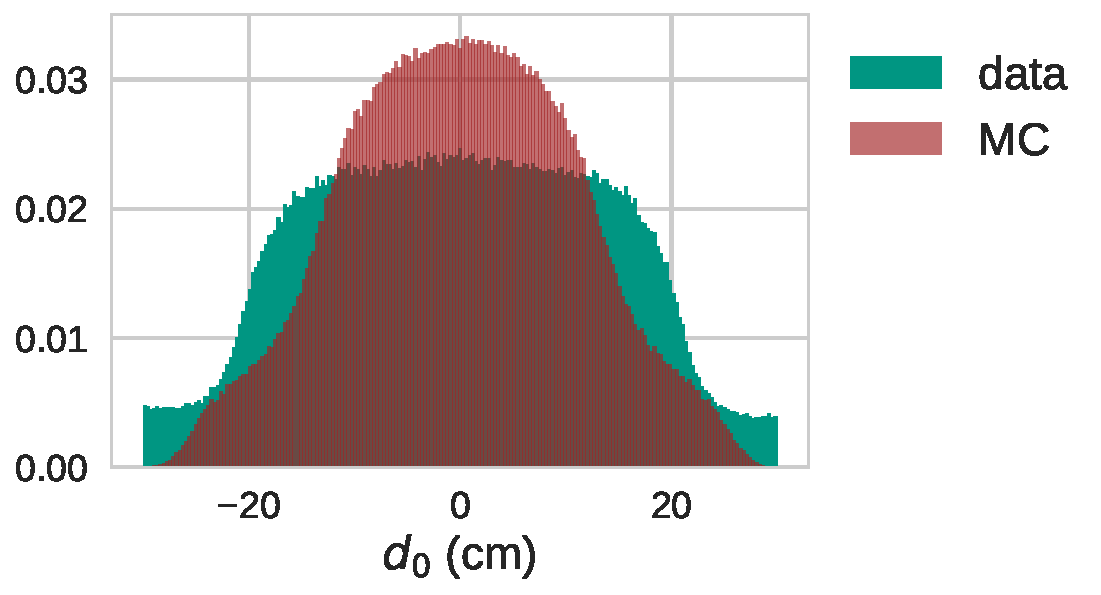
\includegraphics[width=0.45\textwidth]{figures/gcr_august_2017_d0_distribution.pdf}
  \includegraphics[width=0.45\textwidth]{figures/gcr_august_2017_z0_distribution.pdf}\\
    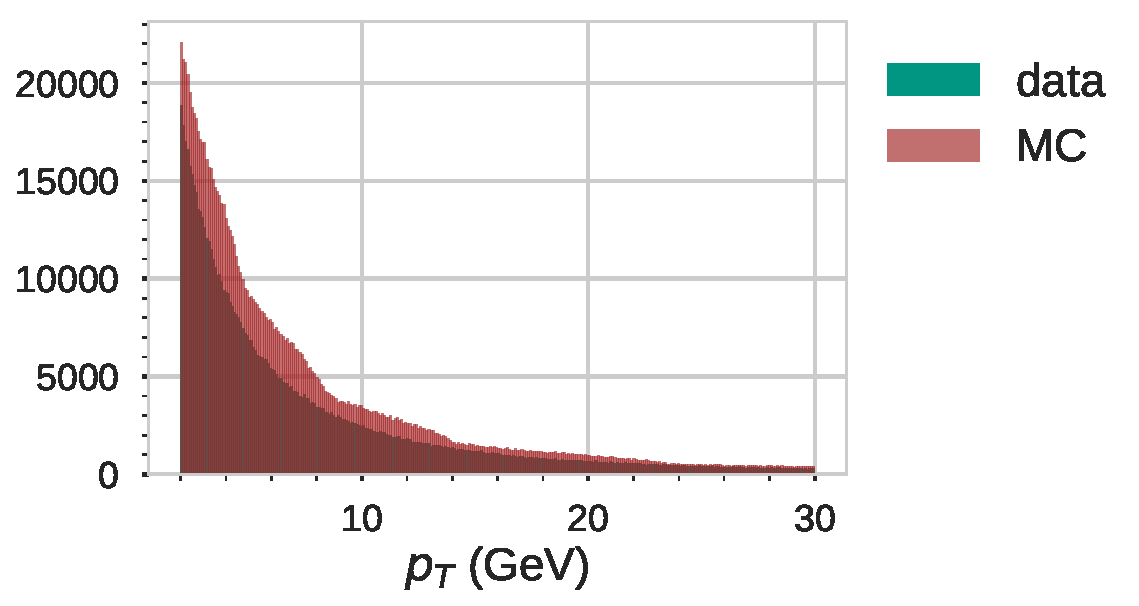
\includegraphics[width=0.45\textwidth]{figures/gcr_august_2017_pt_distribution.pdf}
    \includegraphics[width=0.45\textwidth]{figures/gcr_august_2017_tan_lambda_distribution.pdf}
    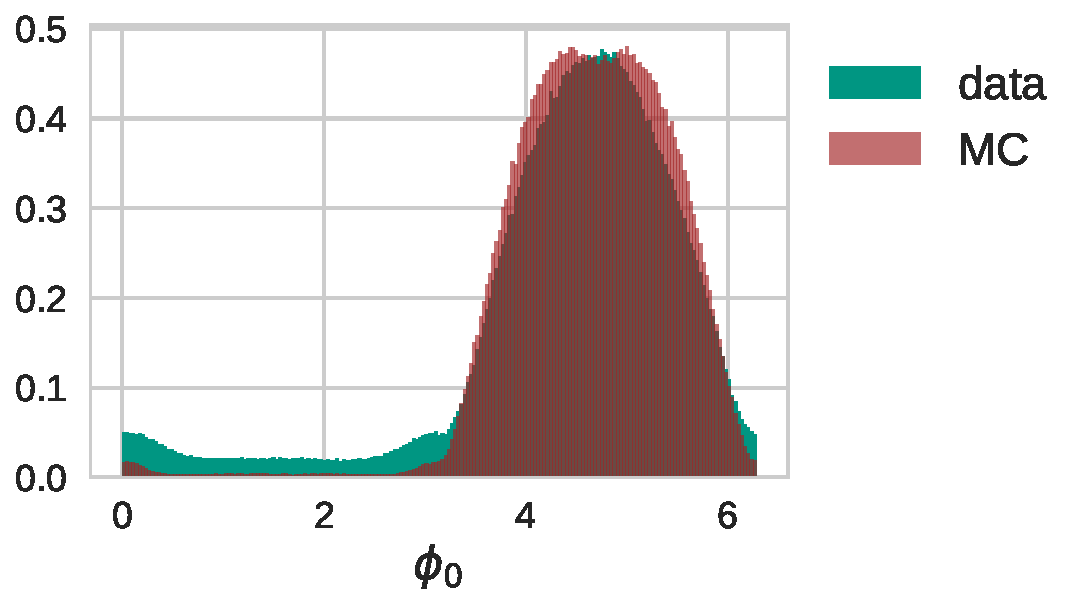
\includegraphics[width=0.45\textwidth]{figures/gcr_august_2017_phi0_distribution.pdf}\\
\end{frame}

\end{document}

%%% Local Variables:
%%% mode: latex
%%% TeX-master: t
%%% End:
